\documentclass{optica-article}

\journal{opticajournal} % for journals or Optica Open

\articletype{Research Article}

\usepackage{lineno}
\linenumbers % Turn off line numbering for Optica Open preprint submissions.

\begin{document}

\title{Universal manuscript template for Optica Publishing Group journals}

\author{Author One,\authormark{1} Author Two,\authormark{2,*} and Author Three\authormark{2,3}}

\address{\authormark{1}Peer Review, Publications Department, Optica Publishing Group, 2010 Massachusetts Avenue NW, Washington, DC 20036, USA\\
\authormark{2}Publications Department, Optica Publishing Group, 2010 Massachusetts Avenue NW, Washington, DC 20036, USA\\
\authormark{3}Currently with the Department of Electronic Journals, Optica Publishing Group, 2010 Massachusetts Avenue NW, Washington, DC 20036, USA}

\email{\authormark{*}opex@optica.org} %% email address is required; see note below about the corresponding author designation

% use {asbstract*} to suppress the copyright line. Copyright information will be added in production

\begin{abstract*} 
\LaTeX{} manuscripts submitted to Optica Publishing Group journals may use these instructions and this universal template format. The template simplifies manuscript preparation and eases transfer between journals. \emph{Applied Optics}, JOSA A, JOSA B, \emph{Journal of Optical Communications and Networking}, \emph{Optica Quantum}, and \emph{Photonics Research} authors should use the length-check template if a precise length estimate is needed. \emph{Optics Letters} authors and authors of short \emph{Optica} articles are encouraged to use the length-check template. Authors using this universal template will still need to adhere to article-length restrictions based on the final, published format. Authors may also \href{https://opticaopen.org}{submit articles} prepared using this template to the Optica Publishing Group preprint server, \href{https://preprints.opticaopen.org}{Optica Open}. However, doing so is optional. Please refer to the submission guidelines found there. Note that copyright and licensing information should no longer be added to your Journal or Optica Open manuscript.

\end{abstract*}

%%%%%%%%%%%%%%%%%%%%%%%%%%  body  %%%%%%%%%%%%%%%%%%%%%%%%%%
\section{Introduction}
Adherence to the specifications listed in this template is essential for efficient review and publication of submissions. Proper reference format is especially important (see Section \ref{sec:refs}). For submissions to the Optica Open preprint server, many of the style and format guidelines described in this template are not applicable, although adhering to the instructions in this template will ease the process to convert a preprint to an Optica Publishing Group journal submission.

\section{Corresponding author}

We require manuscripts to identify a single corresponding author. The corresponding author typically is the person who submits the manuscript and handles correspondence throughout the peer review and publication process. 

\begin{verbatim}
\author{Author One\authormark{1} and Author Two\authormark{2,*}}

\address{\authormark{1}Peer Review, Publications Department,
Optica Publishing Group, 2010 Massachusetts Avenue NW,
Washington, DC 20036, USA\\
\authormark{2}Publications Department, Optica Publishing Group,
2010 Massachusetts Avenue NW, Washington, DC 20036, USA\\

\email{\authormark{*}xyz@optica.org}
\end{verbatim}

This format will generate the following appearance:  

\bigskip

\author{Author One\authormark{1} and Author Two\authormark{2,*}}

\address{\authormark{1}Peer Review, Publications Department,
Optica Publishing Group, 2010 Massachusetts Avenue NW,
Washington, DC 20036, USA\\
\authormark{2}Publications Department, Optica Publishing Group,
2010 Massachusetts Avenue NW, Washington, DC 20036, USA\\
%\authormark{3}xyz@optica.org}

\email{\authormark{*}xyz@optica.org}}

\medskip

If other statements about author contribution and contact are needed, they can be added in addition to the corresponding author designation.
\begin{verbatim}
\author{Author One\authormark{1,$\dag$} and Author Two\authormark{2,$\dag$,*}}

\address{\authormark{1}Peer Review, Publications Department,
Optica Publishing Group, 2010 Massachusetts Avenue NW,
Washington, DC 20036, USA\\
\authormark{2}Publications Department, Optica Publishing Group,
2010 Massachusetts Avenue NW, Washington, DC 20036, USA\\
\authormark{$\dag$}The authors contributed equally to this work.\\
\authormark{*}xyz@optica.org}}
\end{verbatim}

This format will generate the following appearance:

\medskip

\author{Author One\authormark{1,\dag} and Author Two\authormark{2,\dag,*}}

\address{\authormark{1}Peer Review, Publications Department,
Optica Publishing Group, 2010 Massachusetts Avenue NW, Washington, DC 20036, USA\\
\authormark{2}Publications Department, Optica Publishing Group, 2010 Massachusetts Avenue NW, Washington, DC 20036, USA\\
\authormark{\dag}The authors contributed equally to this work.\\
\authormark{*}xyz@optica.org}
\medskip

\section{Abstract}
The abstract should be limited to approximately 100 words. If the work of another author is cited in the abstract, that citation should be written out without a number, (e.g., journal, volume, first page, and year in square brackets [Opt. Express {\bfseries 22}, 1234 (2014)]), and a separate citation should be included in the body of the text. The first reference cited in the main text must be [1]. Do not include numbers, bullets, or lists inside the abstract. Note that no licensing or copyright statement should appear on the manuscript itself. Such information will be added to the Accepted Manuscript, the published version, or the Optica Open preprint as part of production to ensure accuracy and consistency of appearance.

\begin{figure}[ht!]
\centering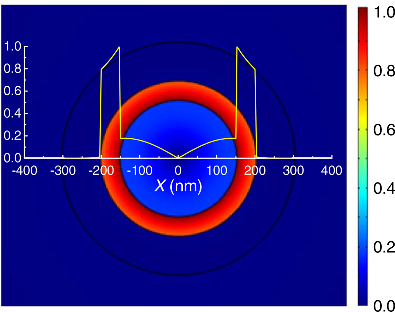
\includegraphics[width=7cm]{opticafig1}
\caption{Sample caption (Fig. 2, \cite{Yelin:03}).}
\end{figure}


\section{Assessing final manuscript length}
The Universal Manuscript Template is based on the Express journal layout and will provide an accurate length estimate for \emph{Optics Express}, \emph{Biomedical Optics Express},  \emph{Optical Materials Express}, \emph{Optica Quantum}, and \emph{Optics Continuum}. \emph{Applied Optics}, JOSAA, JOSAB, \emph{Optics Letters}, \emph{Optica}, \emph{Optica Quantum}, \emph{Optics Continuum}, and \emph{Photonics Research} publish articles in a two-column layout. To estimate the final page count in a two-column layout, multiply the manuscript page count (in increments of 1/4 page) by 60\%. For example, 11.5 pages in the Universal Manuscript Template are roughly equivalent to 7 composed two-column pages. Note that the estimate is only an approximation, as treatment of figure sizing, equation display, and other aspects can vary greatly across manuscripts. Authors of Letters may use the legacy template for a more accurate length estimate.

\section{Figures, tables, and supplementary materials}

\subsection{Figures and tables}
Figures and tables should be placed in the body of the manuscript. Standard \LaTeX{} environments should be used to place tables and figures:
\begin{verbatim}
\begin{figure}[htbp]
\centering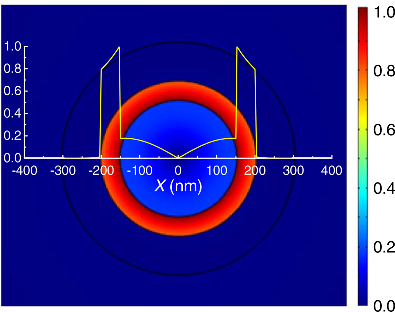
\includegraphics[width=7cm]{opticafig1}
\caption{Sample caption (Fig. 2, \cite{Yelin:03}).}
\end{figure}
\end{verbatim}

\subsection{Supplementary materials in Optica Publishing Group journals}
Our journals allow authors to include supplementary materials as integral parts of a manuscript. Such materials are subject to peer-review procedures along with the rest of the paper and should be uploaded and described using our Prism manuscript system. Please refer to the \href{https://opg.optica.org/submit/style/supplementary_materials.cfm}{Author Guidelines for Supplementary Materials in Optica Publishing Group Journals} for more detailed instructions on labeling supplementary materials and your manuscript. For preprints submitted to Optica Open a link to supplemental material should be included in the submission, but do not upload the material.

\textbf{Authors may also include Supplemental Documents} (PDF documents with expanded descriptions or methods) with the primary manuscript. At this time, supplemental PDF files are not accepted for partner titles, JOCN and \emph{Photonics Research}. To reference the supplementary document, the statement ``See Supplement 1 for supporting content.'' should appear at the bottom of the manuscript (above the References heading). Supplemental documents are not accepted for Optica Open preprints.

\subsection{Sample Dataset Citation}

1. M. Partridge, "Spectra evolution during coating," figshare (2014), http://dx.doi.org/10.6084/m9.figshare.1004612.

\subsection{Sample Code Citation}

2. C. Rivers, "Epipy: Python tools for epidemiology," figshare (2014) [retrieved 13 May 2015], http://dx.doi.org/10.6084/m9.figshare.1005064.



\section{Mathematical and scientific notation}

\subsection{Displayed equations} Displayed equations should be centered.
Equation numbers should appear at the right-hand margin, in
parentheses:
\begin{equation}
J(\rho) =
 \frac{\gamma^2}{2} \; \sum_{k({\rm even}) = -\infty}^{\infty}
	\frac{(1 + k \tau)}{ \left[ (1 + k \tau)^2 + (\gamma  \rho)^2  \right]^{3/2} }.
\end{equation}

All equations should be numbered in the order in which they appear
and should be referenced  from within the main text as Eq. (1),
Eq. (2), and so on [or as inequality (1), etc., as appropriate].

\section{Backmatter}

Backmatter sections should be listed in the order Funding/Acknowledgment/Disclosures/Data Availability Statement/Supplemental Document section. An example of backmatter with each of these sections included is shown below.

\begin{backmatter}
\bmsection{Funding}
Content in the funding section will be generated entirely from details submitted to Prism. Authors may add placeholder text in the manuscript to assess length, but any text added to this section in the manuscript will be replaced during production and will display official funder names along with any grant numbers provided. If additional details about a funder are required, they may be added to the Acknowledgments, even if this duplicates information in the funding section. See the example below in Acknowledgements. For preprint submissions, please include funder names and grant numbers in the manuscript.

\bmsection{Acknowledgments}
The section title should not follow the numbering scheme of the body of the paper. Additional information crediting individuals who contributed to the work being reported, clarifying who received funding from a particular source, or other information that does not fit the criteria for the funding block may also be included; for example, ``K. Flockhart thanks the National Science Foundation for help identifying collaborators for this work.'' 

\bmsection{Disclosures}
Disclosures should be listed in a separate nonnumbered section at the end of the manuscript. List the Disclosures codes identified on the \href{https://opg.optica.org/submit/review/conflicts-interest-policy.cfm}{Conflict of Interest policy page}, as shown in the examples below:

\medskip

\noindent ABC: 123 Corporation (I,E,P), DEF: 456 Corporation (R,S). GHI: 789 Corporation (C).

\medskip

\noindent If there are no disclosures, then list ``The authors declare no conflicts of interest.''


\bmsection{Data Availability Statement}
A Data Availability Statement (DAS) will be required for all submissions beginning 1 March 2021. The DAS should be an unnumbered separate section titled ``Data Availability'' that
immediately follows the Disclosures section. See the \href{https://opg.optica.org/submit/review/data-availability-policy.cfm}{Data Availability Statement policy page} for more information.

Optica has identified four common (sometimes overlapping) situations that authors should use as guidance. These are provided as minimal models, and authors should feel free to
include any additional details that may be relevant.

\begin{enumerate}
\item When datasets are included as integral supplementary material in the paper, they must be declared (e.g., as "Dataset 1" following our current supplementary materials policy) and cited in the DAS, and should appear in the references.

\bmsection{Data availability} Data underlying the results presented in this paper are available in Dataset 1, Ref. [3].

\bigskip

\item When datasets are cited but not submitted as integral supplementary material, they must be cited in the DAS and should appear in the references.

\bmsection{Data availability} Data underlying the results presented in this paper are available in Ref. [3].

\bigskip

\item If the data generated or analyzed as part of the research are not publicly available, that should be stated. Authors are encouraged to explain why (e.g.~the data may be restricted for privacy reasons), and how the data might be obtained or accessed in the future.

\bmsection{Data availability} Data underlying the results presented in this paper are not publicly available at this time but may be obtained from the authors upon reasonable request.

\bigskip

\item If no data were generated or analyzed in the presented research, that should be stated.

\bmsection{Data availability} No data were generated or analyzed in the presented research.
\end{enumerate}

\bigskip

\noindent Data availability statements are not required for preprint submissions.

\bmsection{Supplemental document}
See Supplement 1 for supporting content. 

\end{backmatter}

\section{References}
\label{sec:refs}
Proper formatting of references is extremely important, not only for consistent appearance but also for accurate electronic tagging. Please follow the guidelines provided below on formatting, callouts, and use of Bib\TeX.

\subsection{Formatting reference items}
Each source must have its own reference number. Footnotes (notes at the bottom of text pages) are not used in our journals. List up to three authors, and if there are more than three use \emph{et al.} after that. Examples of common reference types can be found in the  \href{https://opg.optica.org/jot/submit/style/oestyleguide.cfm} {style guide}.


The commands \verb+\begin{thebibliography}{}+ and \verb+\end{thebibliography}+ format the section according to standard style, showing the title {\bfseries References}.  Use the \verb+\bibitem{label}+ command to start each reference.

\subsection{Formatting reference citations}
References should be numbered consecutively in the order in which they are referenced in the body of the paper. Set reference callouts with standard \verb+\cite{}+ command or set manually inside square brackets [1].

To reference multiple articles at once, simply use a comma to separate the reference labels, e.g. \verb+\cite{Yelin:03,Masajada:13,Zhang:14}+, produces \cite{Yelin:03,Masajada:13,Zhang:14}.
%Using the \texttt{cite.sty} package will make these citations appear like so: [2--4].

\subsection{Bib\TeX}
\label{sec:bibtex}
Bib\TeX{} may be used to create a file containing the references, whose contents (i.e., contents of \texttt{.bbl} file) can then be pasted into the bibliography section of the \texttt{.tex} file. A Bib\TeX{} style file, \texttt{opticajnl.bst}, is provided.

If your manuscript already contains a manually formatted \verb|\begin{thebibliography}|... \verb|\end{thebibliography}| list, then delete the \texttt{latexmkrc} file (if present) from your submission files. However you should ensure that your manually-formatted reference list adheres to style accurately.

\section{Conclusion}
After proofreading the manuscript, compress your .tex manuscript file and all figures (which should be in EPS or PDF format) in a ZIP, TAR or TAR-GZIP package. All files must be referenced at the root level (e.g., file \texttt{figure-1.eps}, not \texttt{/myfigs/figure-1.eps}). If there are supplementary materials, the associated files should not be included in your manuscript archive but be uploaded separately through the Prism interface.

%%%%%%%%%%%%%%%%%%%%%%% References %%%%%%%%%%%%%%%%%%%%%%%%%

Add references with BibTeX or manually.
\cite{Zhang:14,OPTICA,FORSTER2007,Dean2006,testthesis,Yelin:03,Masajada:13,codeexample}

%%%%%%%%%% If using BibTeX:
\bibliography{sample}

%%%%%%%%%% If preparing manually:
% \begin{thebibliography}{1}
% \newcommand{\enquote}[1]{``#1''}

% \bibitem{Zhang:14}
% Y.~Zhang, S.~Qiao, L.~Sun, Q.~W. Shi, W.~Huang, L.~Li, and Z.~Yang,
%   \enquote{Photoinduced active terahertz metamaterials with nanostructured
%   vanadium dioxide film deposited by sol-gel method,}
%   {\protect\JournalTitle{Optics Express}} \textbf{22}, 11070--11078 (2014).

% \bibitem{Optica}
% {Optica}, \enquote{{Optica Publishing Group},}
%   \url{http://www.opg.optica.org}.

% \bibitem{FORSTER2007}
% P.~Forster, V.~Ramaswamy, P.~Artaxo, T.~Bernsten, R.~Betts, D.~Fahey,
%   J.~Haywood, J.~Lean, D.~Lowe, G.~Myhre, J.~Nganga, R.~Prinn, G.~Raga,
%   M.~Schulz, and R.~V. Dorland, \enquote{Changes in atmospheric consituents and
%   in radiative forcing,} in \enquote{Climate Change 2007: The Physical Science
%   Basis. Contribution of Working Group 1 to the Fourth assesment report of
%   Intergovernmental Panel on Climate Change,}  S.~Solomon, D.~Qin, M.~Manning,
%   Z.~Chen, M.~Marquis, K.~B. Averyt, M.~Tignor, and H.~L. Miler, eds.
%   (Cambridge University Press, 2007).

% \end{thebibliography}

\end{document}